% !TeX program = pdflatex
\documentclass[border=6pt]{standalone}
\usepackage{tikz}
\usetikzlibrary{arrows.meta, positioning, calc}

\definecolor{MediumRed}{rgb}{0.925, 0.345, 0.345}
\definecolor{MediumGreen}{rgb}{0.37, 0.7, 0.66}
\definecolor{MediumBlue}{rgb}{0.015, 0.315, 0.45}
\definecolor{DarkBlue}{rgb}{0.05, 0.15, 0.35}

\def\s{0.30} % cm por punto BLEU-4

\begin{document}
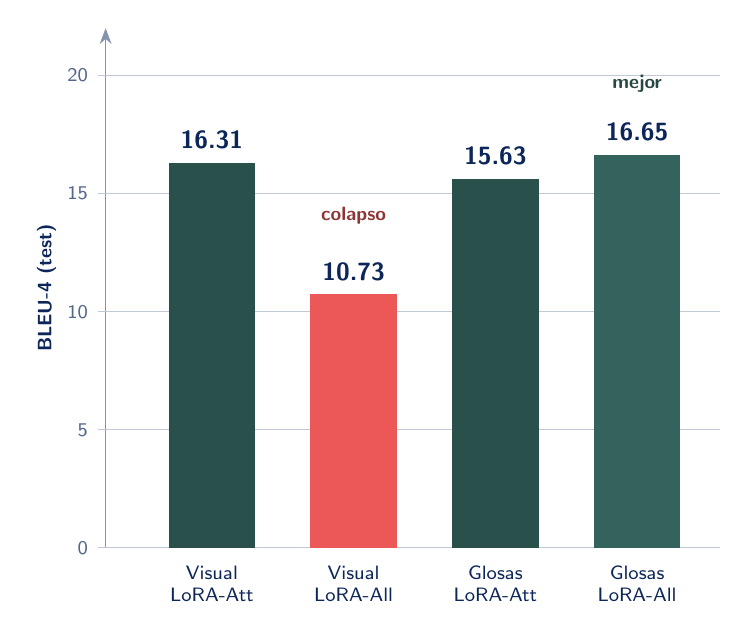
\begin{tikzpicture}[font=\sffamily]

% eje y
\draw[DarkBlue!50, -{Stealth[length=2mm]}] (-0.4,0) -- (-0.4,{22*\s});
\foreach \y in {0,5,10,15,20}{
    \draw[DarkBlue!25] (-0.5,{\y*\s}) -- (7.4,{\y*\s});
    \node[font=\sffamily\scriptsize, text=DarkBlue!70, anchor=east] at (-0.5,{\y*\s}) {\y};
}
\node[font=\sffamily\scriptsize\bfseries, text=DarkBlue, rotate=90] at (-1.15,{11*\s}) {BLEU-4 (test)};

% barras: x/valor/color/etiqueta1/etiqueta2
\foreach \x/\v/\c/\la/\lb in {%
    0.4/16.31/MediumGreen!45!black/Visual/LoRA-Att,
    2.2/10.73/MediumRed/Visual/LoRA-All,
    4.0/15.63/MediumGreen!45!black/Glosas/LoRA-Att,
    5.8/16.65/MediumGreen!55!black/Glosas/LoRA-All}{%
    \fill[\c] (\x,0) rectangle (\x+1.1,{\v*\s});
    \node[font=\sffamily\small\bfseries, text=DarkBlue, anchor=south] at (\x+0.55,{\v*\s+0.05}) {\v};
    \node[font=\sffamily\scriptsize, text=DarkBlue, anchor=north, align=center] at (\x+0.55,-0.1)
        {\la\\\lb};
}

% resaltar colapso y mejor
\node[font=\sffamily\scriptsize\bfseries, text=MediumRed!60!black, align=center] at (2.75,{10.73*\s+1.0})
    {colapso};
\node[font=\sffamily\scriptsize\bfseries, text=MediumGreen!40!black] at (6.35,{16.65*\s+0.9}) {mejor};

\end{tikzpicture}
\end{document}
